\documentclass[lang=cn,10pt,bibend=bibtex]{elegantbook}

\title{10月份科研报告}

\author{Wenchong Huang}
\date{Oct. 10, 2023}

\setcounter{tocdepth}{3}

\logo{logo-blue.jpg}
\cover{cover.jpeg}
\usepackage{multirow}
\usepackage{xpatch}
\makeatletter
\xpatchcmd{\chapter}
  {\if@openright\cleardoublepage\else\clearpage\fi}{\par\relax}
  {}{}
\makeatother

% 本文档命令
\usepackage{array, float}
\newcommand{\ccr}[1]{\makecell{{\color{#1}\rule{1cm}{1cm}}}}

% 修改标题页的橙色带
% \definecolor{customcolor}{RGB}{32,178,170}
% \colorlet{coverlinecolor}{customcolor}

\begin{document}

\maketitle
\frontmatter

\tableofcontents

\mainmatter

\chapter{分离方法}

\section{分离方法介绍}

假设我们有初值问题:
\begin{equation}
    \frac{d\phi}{dt}=A(\phi)+B(\phi),\quad \phi(0)=\phi_0.
\end{equation}

我们有求解器$\mathcal{N}_A(\phi_0,T)$,它输出初值问题
\begin{equation}
    \frac{d\phi}{dt}=A(\phi),\quad \phi(0)=\phi_0.
\end{equation}

在$T$时刻的解。同时也有求解器$\mathcal{N}_B(\phi_0,T)$,它输出初值问题
\begin{equation}
    \frac{d\phi}{dt}=B(\phi),\quad \phi(0)=\phi_0.
\end{equation}

在$T$时刻的解。我们可以借助这两个求解器构造一个分离格式,例如:
\begin{align*}
    \phi^\star &= \mathcal{N}_A(\phi_n,k),\\
    \phi_{n+1} &= \mathcal{N}_B(\phi^\star,k).
\end{align*}

这个格式有两个性质:
\begin{enumerate}
    \item 只要求解器$\mathcal{N}_A$与$\mathcal{N}_B$收敛,那么分离格式也收敛;
    \item 不论求解器$\mathcal{N}_A$与$\mathcal{N}_B$的精度有多高,在一些特定问题中,该分离格式也只有一阶精度。例如当$A,B$是不交换的线性算子时,可以证明:即使求解器都是精确的,其单步误差也将达到$O(k^2)$。
\end{enumerate}

\section{二阶时间离散:Strang Splitting}

我们沿用(1.1)(1.2)(1.3)式的符号。Strang Splitting格式\cite{Strang1968}如下:
\begin{align*}
    \phi^\star &= \mathcal{N}_A(\phi_n,k/2),\\
    \phi^{\star\star} &= \mathcal{N}_B(\phi^\star,k),\\
    \phi_{n+1} &= \mathcal{N}_A(\phi^{\star\star},k/2).
\end{align*}

为方便后文的表述,我们记由Strang Splitting格式算一步得到的解为:
\begin{equation}
    \phi_{n+1} = S(\phi_n,k).
\end{equation}

\section{四阶时间离散:Forest-Ruth splitting}

我们沿用(1.4)式的符号。Forest-Ruth Splitting格式\cite{Forest1990}如下:
\begin{align*}
    \phi^\star &= S(\phi_n,\omega_1k),\\
    \phi^{\star\star} &= S(\phi^\star,\omega_2k),\\
    \phi_{n+1} &= S(\phi^{\star\star},\omega_1k).
\end{align*}

其中
\begin{equation*}
    \omega_1=\frac{1}{2-2^{1/3}},\quad \omega_2=-\frac{2^{1/3}}{2-2^{1/3}}
\end{equation*}

众所周知,扩散方程的逆过程是不稳定的,而这个格式中居然出现了负时间步,它将会是万恶之源。

\section{四阶紧致时间离散:Chin splitting}

我们沿用(1.1)(1.2)(1.3)式的符号。同时我们设求解器$\mathcal{N}_C(\phi_0,\tau,T)$输出初值问题
\begin{equation}
    \frac{d\phi}{dt}=A(\phi)+\frac{\tau^2}{48}(2ABA-AAB-BAA)(\phi),\quad \phi(0)=\phi_0.
\end{equation}

在$T$时刻的解。Chin Splitting格式\cite{Chin1997}如下:
\begin{align*}
    \phi^{(1)} &= \mathcal{N}_A(\phi_n,k/6),\\
    \phi^{(2)} &= \mathcal{N}_B(\phi^{(1)},k/2),\\
    \phi^{(2)} &= \mathcal{N}_C(\phi^{(2)},k,2k/3),\\
    \phi^{(4)} &= \mathcal{N}_B(\phi^{(3)},k/2),\\
    \phi_{n+1} &= \mathcal{N}_A(\phi^{(4)},k/6).
\end{align*}

当
\begin{equation}
    2ABA-AAB-BAA=0
\end{equation}

时,这是一个相当好的格式。

\vspace{5em}

\chapter{谱方法}

\vspace{-1em}

\section{热方程的谱方法}

\subsection{方法描述}

考虑$[0,1]^2$上的周期边界热方程
\begin{equation*}
    \frac{\partial \phi}{\partial t}=\Delta \phi.
\end{equation*}

对$\phi$做离散傅里叶变换,得到
\begin{equation*}
    \phi(x,y,t)\approx \frac{1}{(2N+1)^2} \sum_{n,m=-N}^N \hat{\phi}_{n,m}(t)e^{-2\pi\mathbf{i}(nx+my)}.
\end{equation*}

代入热方程,即得
\begin{equation*}
    \frac{d \hat{\phi}_{n,m}}{d t}=-4\pi^2(n^2+m^2) \hat{\phi}_{n,m},\qquad n,m=-N,...,N.
\end{equation*}

这些ODE可以独立求解,得到
\begin{equation}
    \hat{\phi}_{n,m}(t)=\exp(-4\pi^2(n^2+m^2)) \hat{\phi}_{n,m}(0),\qquad n,m=-N,...,N.
\end{equation}

于是我们得到谱方法:
\begin{enumerate}
    \item 对$\phi(x_j,y_k,0)(j,k=0,...,2N)$做离散傅里叶变换得到$\hat{\phi}_{n,m}(0)(n,m=-N,...,N)$.
    \item 由(2.1)式计算$\hat{\phi}_{n,m}(t)(n,m=-N,...,N)$.
    \item 对$\hat{\phi}_{n,m}(t)(n,m=-N,...,N)$做离散傅里叶逆变换得到$\phi(x_j,y_k,t)(j,k=0,...,2N)$。
\end{enumerate}

其中$x_j=\frac{j}{2N+1},y_k=\frac{k}{2N+1}$。朴素的谱方法要求边界必须满足周期条件,并且必须使用规则等分网格。

\subsection{数值算例}

我们取初始条件
\begin{equation}
    \phi_0(x,y)=\exp((-(x-0.5)^2-(y-0.5)^2)\times 60).
\end{equation}

求方程在$T=0.05$时刻的解,测试结果如下表,误差由Richardson外插法估计(注意时间单位为\textbf{毫秒},且运行时间不包含初始化时间)。

\begin{table}[H]
    \centering
    \small
    \begin{tabular}{c|cccc}
    \textbf{$M$}              & 64           & 128          & 256          & 512   \\ \hline
    1范数误差                  & 1.04517e-13   & 7.09259e-13   & 9.18621e-13  & 2.63755e-14 \\
    2范数误差                  & 1.14391e-13   & 7.10592e-13   & 9.19695e-13  & 3.28119e-14 \\
    $\infty$范数误差           & 2.25001e-13   & 8.25000e-13   & 1.05000e-12  & 1.00017e-13 \\
    运行时间(\textbf{ms})                & 0.0502              & 0.302             & 0.788          & 4.18
    \end{tabular}
    \caption{谱方法解热方程的测试结果}
\end{table}

这些误差几乎都是舍入误差的累积,因此无法算收敛阶。

\vspace{-.5em}

\section{对流扩散方程的有限体-谱分离方法}

\vspace{-.5em}

\subsection{方法描述}

考虑$[0,1]^2$上的周期边界对流扩散方程
\begin{equation*}
    \frac{\partial \phi}{\partial t}=\nabla\cdot(\mathbf{u}\phi)+\nu \Delta\phi.
\end{equation*}

设求解器$\mathcal{N}_A(\phi_0,T)$它输出初值问题
\begin{equation}
    \frac{d\phi}{dt}=\nabla\cdot(\mathbf{u}\phi),\quad \phi(0)=\phi_0.
\end{equation}

在$T$时刻的解。具体地,我们对$\phi$做有限体积离散,然后对流算子做四阶有限体积离散,时间上再采用经典RK方法。设求解器$\mathcal{N}_B(\phi_0,T)$它输出初值问题
\begin{equation}
    \frac{d\phi}{dt}=\nu \Delta\phi,\quad \phi(0)=\phi_0.
\end{equation}

在$T$时刻的解,内部采用谱方法。

最后采用Forest-Ruth Splitting或者Chin Splitting将二者耦合。其中(1.5)式的求解器$\mathcal{N}_C$由$\mathcal{N}_A$替代,但注意到对流扩散方程不满足(1.6)式,因此这个替代是不精确的,可能导致Chin Splitting掉阶。

\vspace{-.5em}

\subsection{数值算例}

我们取$\nu=0.001$,及初始条件
\begin{equation}
    \phi_0(x,y)=\exp((-(x-0.5)^2-(y-0.75)^2)\times 100\log(10^{16})).
\end{equation}

也就是《数学实践》课程大作业的第二个算例。在$T=10$时刻,其数值解如下图所示。

\vspace{-1em}
\begin{figure}[H]
    \centering
    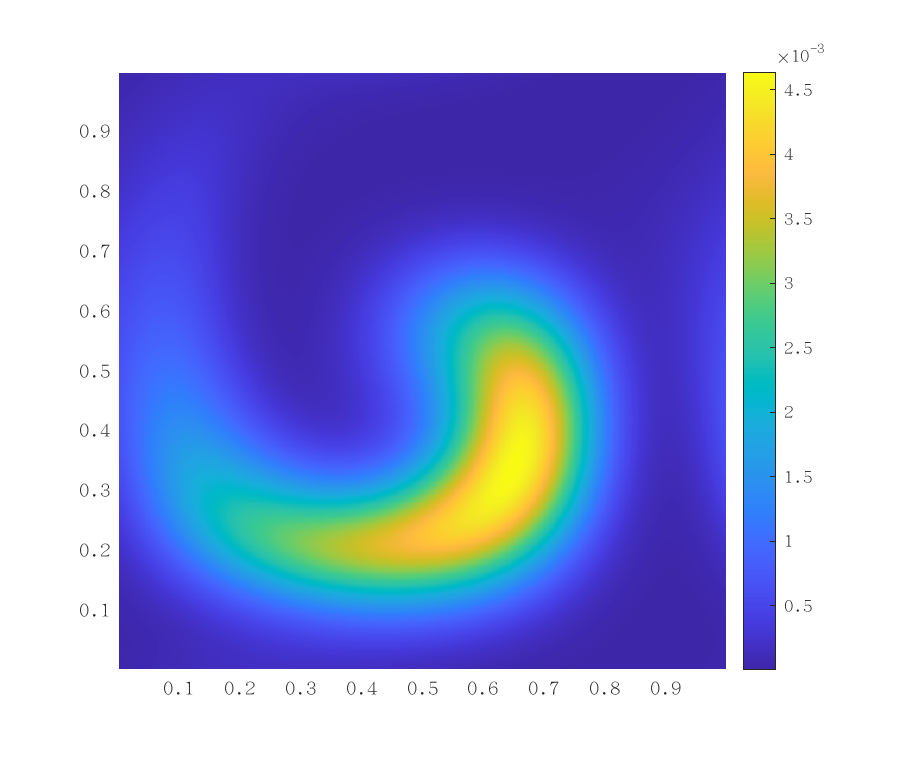
\includegraphics[width=0.5\textwidth]{eps/AdvDif.eps}
\end{figure}

测试结果如下表。

\begin{table}[H]
    \centering
    \small
    \begin{tabular}{c|ccccccc}
    \textbf{$M$}              & 64          & 收敛阶 & 128         & 收敛阶 & 256         & 收敛阶 & 512   \\ \hline
    1范数误差                  & 9.74830e-08 & 3.98  & 6.18924e-09 & 3.99  & 3.88379e-10 &  4.00 & 2.42993e-11 \\
    2范数误差                  & 1.75527e-07 & 3.98  & 1.11599e-08 & 3.99  & 7.00492e-10 &  4.00 & 4.38596e-11 \\
    $\infty$范数误差           & 7.90676e-07 & 3.94  & 5.16717e-08 & 3.99  & 3.26315e-09 &  3.99 & 2.05022e-10 \\
    运行时间(s)                & 5           &       & 41          &       & 390         &       & 3503
    \end{tabular}
    \caption{当时大作业的测试结果}
\end{table}

\begin{table}[H]
    \centering
    \small
    \begin{tabular}{c|ccccccc}
    \textbf{$M$}              & 64          & 收敛阶 & 128         & 收敛阶 & 256         & 收敛阶 & 512   \\ \hline
    1范数误差                  & 9.81486e-08 & 3.98  & 6.22740e-09 &  - & 无法估计误差 &  - & - \\
    2范数误差                  & 1.74020e-07 & 3.98  & 1.10630e-08 &  - & 无法估计误差 &  - & - \\
    $\infty$范数误差           & 8.14289e-07 & 3.97  & 5.20873e-08 &  - & 无法估计误差 &  - & - \\
    运行时间(s)                & 0.103           &       & 0.854          &       & 8.96         &       & -
    \end{tabular}
    \caption{Forest-Ruth Splitting的测试结果}
\end{table}

\begin{table}[H]
    \centering
    \small
    \begin{tabular}{c|ccccccc}
    \textbf{$M$}              & 64          & 收敛阶 & 128         & 收敛阶 & 256         & 收敛阶 & 512   \\ \hline
    1范数误差                  & 9.73896e-08 & 4.00  & 6.07244e-09 & 3.96  & 3.91085e-10 &  3.02 & 4.81695e-11 \\
    2范数误差                  & 1.72842e-07 & 4.00  & 1.07871e-08 & 4.00  & 6.75903e-10 &  3.13 & 7.69678e-11 \\
    $\infty$范数误差           & 8.04398e-07 & 3.98  & 5.08533e-08 & 3.87  & 3.48553e-09 &  3.35 & 3.42374e-10 \\
    运行时间(s)                & 0.0515          &       & 0.517          &       & 4.56         &       & 50.6
    \end{tabular}
    \caption{Chin Splitting的测试结果}
\end{table}

从时间上看,比起当时的大作业,运算速度有了质的飞跃。

不过,Forest-Ruth Splitting最多只能算到$256$的网格,因为在$512$的网格中,扩散项的负时间步导致了指数爆炸:在一个负时间步中,最高频的谱需要乘约$2\times 10^{37}$,这对浮点精度来说是灾难。

另外,Chin Splitting在256到512时掉阶的原因可能是用$\mathcal{N}_A$代替$\mathcal{N}_C$的原因,也有可能是谱方法的固有误差累积。从上一节的测试,可以发现每次求解都有\verb|1e-13|的固有误差,如果经过多个时间步累积,可能会导致它成为主要的误差来源。

我希望原因是后者,这样$\mathcal{N}_A$代替$\mathcal{N}_C$至少在精度足够高的环境下可行,当然还需要一些理论验证。

\vspace{5em}

\chapter{SAV方法}

\section{Cahn-Hilliard方程的SAV方法}

考虑能量泛函
\begin{equation}
    E[\phi(\mathbf{x})]=\int_\Omega\left(\frac{1}{2}|\nabla \phi|^2+F(\phi)\right)\;d\mathbf{x}.
\end{equation}

以及如下形式的Cahn-Hilliard方程:
\begin{align}
    \frac{\partial \phi}{\partial t}&=\Delta\mu,\\
    \mu&=\frac{\delta E}{\delta\phi}=-\Delta \phi+F'(\phi).
\end{align}

\section{GePUP-SAV-SDIRK}

\vspace{5em}

\printbibliography[heading=bibintoc,title=\ebibname]

\appendix

\newpage

\chapter{二维FFT}

\section{公式推导}

\begin{lemma}
    二维DFT可归结为如下问题:已知二元多项式
    \begin{equation*}
        f(x,y)=\sum_{n=0}^{N-1}\sum_{m=0}^{N-1} a_{n,m}x^ny^m,
    \end{equation*}

    求$f(\omega_N^j,\omega_N^k),(j,k=0,...,N-1)$的值。
\end{lemma}

引理很容易验证,关键是如何快速求解这个问题。为此,我们对多项式做奇偶项划分,即令
\begin{align*}
    p_1(x,y)&=\sum_{n=0}^{N/2-1}\sum_{m=0}^{N/2-1} a_{2n,2m}x^ny^m,\\
    p_2(x,y)&=\sum_{n=0}^{N/2-1}\sum_{m=0}^{N/2-1} a_{2n,2m+1}x^ny^m,\\
    p_3(x,y)&=\sum_{n=0}^{N/2-1}\sum_{m=0}^{N/2-1} a_{2n+1,2m}x^ny^m,\\
    p_4(x,y)&=\sum_{n=0}^{N/2-1}\sum_{m=0}^{N/2-1} a_{2n+1,2m+1}x^ny^m.
\end{align*}

于是我们有
\begin{equation*}
    f(x,y)=p_1(x^2,y^2)+yp_2(x^2,y^2)+xp_3(x^2,y^2)+xyp_4(x^2,y^2).
\end{equation*}

现任取整数$j,k\in[0,N/2)$,注意到
\begin{align*}
    f(\omega_N^j,\omega_N^k)&=p_1(\omega_{N/2}^j,\omega_{N/2}^k)+\omega_N^kp_2(\omega_{N/2}^j,\omega_{N/2}^k)+\omega_N^jp_3(\omega_{N/2}^j,\omega_{N/2}^k)+\omega_N^j\omega_N^kp_4(\omega_{N/2}^j,\omega_{N/2}^k)\\
    f(\omega_N^j,\omega_N^{N/2+k})&=p_1(\omega_{N/2}^j,\omega_{N/2}^k)-\omega_N^kp_2(\omega_{N/2}^j,\omega_{N/2}^k)+\omega_N^jp_3(\omega_{N/2}^j,\omega_{N/2}^k)-\omega_N^j\omega_N^kp_4(\omega_{N/2}^j,\omega_{N/2}^k)\\
    f(\omega_N^{N/2+j},\omega_N^k)&=p_1(\omega_{N/2}^j,\omega_{N/2}^k)+\omega_N^kp_2(\omega_{N/2}^j,\omega_{N/2}^k)-\omega_N^jp_3(\omega_{N/2}^j,\omega_{N/2}^k)-\omega_N^j\omega_N^kp_4(\omega_{N/2}^j,\omega_{N/2}^k)\\
    f(\omega_N^{N/2+j},\omega_N^{N/2+k})&=p_1(\omega_{N/2}^j,\omega_{N/2}^k)-\omega_N^kp_2(\omega_{N/2}^j,\omega_{N/2}^k)-\omega_N^jp_3(\omega_{N/2}^j,\omega_{N/2}^k)+\omega_N^j\omega_N^kp_4(\omega_{N/2}^j,\omega_{N/2}^k)\\
\end{align*}

因此,只要我们先算出
\begin{equation}
    p_i(\omega_{N/2}^j,\omega_{N/2}^k),(j,k=0,...,N/2-1),\quad i=1,2,3,4.
\end{equation}

我们就可以再用$O(N)$的时间完成问题求解。不难看出(A.1)式的形式与原问题完全一致,只是$N$换成了$N/2$。我们设求解原问题的时间复杂度为$T(N)$,有:
\begin{equation*}
    T(N)=4T\left(\frac{N}{2}\right)+\Theta(N)=\Theta(N^2\log N).
\end{equation*}

因此我们可以借助分治实现高效求解。但如果使用递归式写法,我们需要在每一层存储奇偶项划分后$p_1,p_2,p_3,p_4$的各项系数,从而空间复杂度也达到$\Theta(N^2\log N)$。我们可以用蝴蝶变换来避免递归,即自底向上模拟分治过程,空间复杂度可以下降到$\Theta(N^2)$。详见代码\verb|fft2D.cpp|。

\section{FFTW库的使用}

FFTW(FFT in the West)库曾经是世界上最快的FFT库,不过现在Intel用mkl优化后的FFTW要更快。以2维FFT为例,在输入输出均为复数数组的情况下,速度大约是我手写FFT的1.2倍。

注意到一个问题:FFT正变换时,输入数组为实数、输出数组为复数;FFT逆变换时,输入数组为复数、输出数组为实数。FFTW能利用这个性质,进一步优化FFT。下面是一个使用FFTW的例程。

\begin{lstlisting}[language=c++]
    #include <bits/stdc++.h>
    #include <fftw3.h>
    using namespace std;
    
    const int N = 1024;
    
    int main(){
        auto out = (fftw_complex*) fftw_malloc(sizeof(fftw_complex) * N*(N/2+1));
        auto in = (double*) fftw_malloc(sizeof(double) * N*N);
        auto p = fftw_plan_dft_r2c_2d(N, N, in, out, FFTW_MEASURE);
        auto pinv = fftw_plan_dft_c2r_2d(N, N, out, in, FFTW_MEASURE);
    
        for(int i = 0; i < N*N; i++)
            in[i] = (double)rand()/RAND_MAX;
        
        // Run FFT and save to out[]
        fftw_execute(p);
    
        // Run IFFT and save to in[]
        fftw_execute(pinv);
    
        return 0;
    }
\end{lstlisting}

实际测试表明,针对输入输出数组的类型优化后的FFTW,其运行速度是我手写FFT的2.4倍。

\end{document}